\newpage
\section{Wyniki}

Parametry modelu:
\begin{itemize}
	  \item liczba neuronów warstw ukrytych - $100$
	  \item liczba warstw - $2$
	  \item liczba głowic - $100$
	  \item rozmiar batcha - $40$
	  \item czas uczenia - $40h$
	  \item Liczba epok - $6$
	  \item współczynnik uczenia - $0.004$
	  \item liczba kroków czasowych - $50$
	\end{itemize}
	
Nie udało nam się otrzymać wyników zbliżonych do tych osiągniętych podczas konkursu PAN. Sprawdziła się
część elementów z analizy ryzyka, które przewidywaliśmy.

\subsection{Problemy}
\subsubsection{Małe doświadczenie w dziedzinie konstruowania sieci neuronowych}
Było to dla nas pierwsze doświadczenie z sieciami neuronowymi, dlatego znaczną ilość czasu poświęciliśmy na 
zrozumienie tego zagadnienia. Aby zrozumieć samą ideę zaczęliśmy od prostych modeli sieci typu feed forward,
następnie przeszliśmy do sieci rekurencyjnych. W całym procesie nauki musieliśmy zrozumieć,
wszystkie zagadnienia z nimi związane, jak etropia krzyżowa, softmax, propagacja w przód, propagacja wsteczna, 
minimalizacja gradientu itp.

\subsubsection{Długi czas uczenia}
Jedna epoka trwała od kilku do kilkunastu godzin w zależności od ilości danych, co znacząco spowalniało 
prace nad usprawnieniem modelu. 

\subsubsection{Znajomość biblioteki}
Zdobytą wiedzę i pomysł należało przełożyć na kod w Pythonie przy wykorzystaniu biblioteki Pytorch. 
Problem, który rozwiązywaliśmy był w jakimś stopniu niestandardowy, dlatego należało modyfikować 
gotowe narzędzia i odpowiednio komponować z nich kod, często popełniane przy tym błędy prowadziły 
do bardzo stopniowych zmian w kodzie, które oddzielone były długim czasem uczenia na sprawdzenie poprawek.

\subsubsection{Przeuczenie}
Ze względu na specyfikę problemu, którego cechą są bardzo krótkie teksty wejściowe bardzo poważnym 
problemem jest przeuczenie sieci, która
bardzo szybko uczy się tekstów treningowych na pamięć. 

\subsection{Różnice w długości tekstów}
Teksty są bardzo krótkie, dodatkowo różnią się długością. Teksty mają od 1500 do 2600 znaków. 1100 znaków 
różnicy w tym przypadku to aż $43\%$ różnicy w długości. Teoretycznie głowica powinna uczyć się przewidywać znaki dla 
swojego autora i na tekstach treningowych robić to najlepiej w porównaniu do pozostałych głowic dla tekstu 
jej autora ze zbioru testowego. Problemem jest jednak sytuacja wyżej opisana. Kiedy znaków jest tak mało 
możliwa jest sytuacja w której głowica, której teksty są tymi najdłuższymi lepiej uczy się modelu języka od
pozostałych głowic więc skuteczniej przewiduje kolejne znaki dla wszystkich nieznanych teksów.

Popularne modele, które potrafią przewidywać kolejne słowa bądź litery szkolone są przykładowo na danych w postaci licznych 
artykułów z \texttt{Wikipedii}, gdzie liczba danych do wyczuenia jest znacznie większa.

\subsection{Błędy implementacyjne}
Błędy w implementacji sieci, które prowadziły do skrajnie złych wyników i znacznie opóźniały tempo pracy.
\begin{figure}[H]
	\centering
	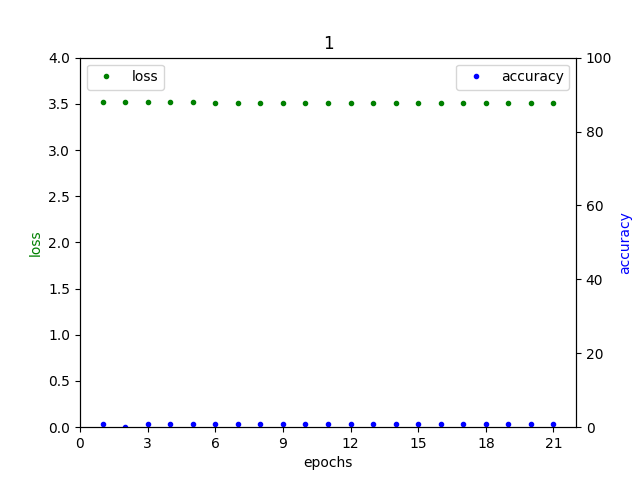
\includegraphics[height=7cm]{./images/result1.png}
	\caption{przykładowe dane z uczenia sieci błędnie zaimplementowanej}
	\label{fig:test5}
	\end{figure}

\subsection{Wyniki eksperymentów}
\TODO{uzupełnić}
